% ============================================================
%  MARITIME AI CHATBOT — RESEARCH & DEPLOYMENT PRESENTATION
%  Professional academic design for supervisor presentation.
%  All slide content stays within borders (adjustbox + shrink).
%  Color palette: Navy #01337D + Gold #C9A227 + clean white.
%  Compiled with pdflatex (TeX Live 2025 Basic).
%  Author: Maritime AI Research Team | March 2026
% ============================================================
\documentclass[aspectratio=169,11pt]{beamer}

% ---- Theme base ----
\usetheme{default}
\useinnertheme{rounded}

% ---- Typography ----
\usepackage{lmodern}
\usepackage[T1]{fontenc}
\usepackage{microtype}
\usefonttheme{professionalfonts}

% ---- Core packages ----
\usepackage{booktabs}
\usepackage{tabularx}
\usepackage{xcolor}
\usepackage{tikz}
\usepackage{amsmath,amssymb}
\usepackage{array}
\usepackage{multirow}
\usepackage{graphicx}
\usepackage{colortbl}
\usepackage{adjustbox}        % Prevents all table/figure overflow — key package
\usepackage{ragged2e}         % RaggedRight inside blocks

\usetikzlibrary{arrows.meta, shapes.geometric, positioning,
                fit, backgrounds, calc, shadings}

% ============================================================
%  COLOUR SYSTEM
% ============================================================
\definecolor{navydeep}{HTML}{01337D}
\definecolor{navymid}{HTML}{1A5276}
\definecolor{navylight}{HTML}{D4E6F1}
\definecolor{gold}{HTML}{C9A227}
\definecolor{goldsoft}{HTML}{F9E79F}
\definecolor{crimson}{HTML}{941B0C}
\definecolor{crimsonsoft}{HTML}{FAEAEA}
\definecolor{amber}{HTML}{B05D0E}
\definecolor{ambersoft}{HTML}{FEF3E2}
\definecolor{forest}{HTML}{1B6B3A}
\definecolor{forestsoft}{HTML}{E8F5EC}
\definecolor{ocean}{HTML}{1565C0}
\definecolor{oceansoft}{HTML}{E3F0FF}
\definecolor{charcoal}{HTML}{1C2B3A}
\definecolor{snow}{HTML}{FAFAFA}
\definecolor{slate}{HTML}{4A5568}

% ============================================================
%  BEAMER COLOR ASSIGNMENTS
% ============================================================
\setbeamercolor{structure}{fg=navydeep}
\setbeamercolor{background canvas}{bg=snow}
\setbeamercolor{normal text}{fg=charcoal}
\setbeamercolor{frametitle}{bg=navydeep, fg=white}
\setbeamercolor{title}{fg=white}
\setbeamercolor{subtitle}{fg=white!85}
\setbeamercolor{section in toc}{fg=navydeep}
\setbeamercolor{item}{fg=navydeep}
\setbeamercolor{subitem}{fg=ocean}
\setbeamercolor{alerted text}{fg=crimson}
\setbeamercolor{example text}{fg=forest}

\setbeamercolor{block title}{bg=navydeep, fg=white}
\setbeamercolor{block body}{bg=navylight, fg=charcoal}
\setbeamercolor{block title alerted}{bg=crimson, fg=white}
\setbeamercolor{block body alerted}{bg=crimsonsoft, fg=charcoal}
\setbeamercolor{block title example}{bg=forest, fg=white}
\setbeamercolor{block body example}{bg=forestsoft, fg=charcoal}

\setbeamercolor{footL}{bg=charcoal,    fg=white!55}
\setbeamercolor{footC}{bg=charcoal!90, fg=white!55}
\setbeamercolor{footR}{bg=charcoal,    fg=gold}
\setbeamercolor{pgbarbg}{bg=charcoal!85}
\setbeamercolor{pgbarfg}{bg=gold}

% ============================================================
%  FONTS
% ============================================================
\setbeamerfont{title}{size=\LARGE, series=\bfseries}
\setbeamerfont{subtitle}{size=\small}
\setbeamerfont{frametitle}{size=\small, series=\bfseries}
\setbeamerfont{block title}{size=\footnotesize, series=\bfseries}
\setbeamerfont{block body}{size=\scriptsize}
\setbeamerfont{section in toc}{size=\normalsize, series=\bfseries}
\setbeamerfont{footfnt}{size=\tiny}

% ============================================================
%  MARGINS
% ============================================================
\setbeamersize{text margin left=0.65cm, text margin right=0.65cm}

% ============================================================
%  FRAMETITLE: navy bar with 4mm gold left accent
%  (uses nested colorboxes — no inline TikZ needed)
% ============================================================
\setbeamertemplate{frametitle}{%
  \nointerlineskip
  \hbox{%
    \begin{beamercolorbox}[wd=4pt, ht=0.80cm, dp=0.15cm]{pgbarfg}%
    \end{beamercolorbox}%
    \begin{beamercolorbox}[wd=\dimexpr\paperwidth-4pt\relax,
                           ht=0.80cm, dp=0.15cm,
                           leftskip=8pt, rightskip=4pt]{frametitle}%
      \usebeamerfont{frametitle}\insertframetitle%
      \ifx\insertframesubtitle\empty\else
        \par\vskip1pt{\color{white!70}\tiny\insertframesubtitle}%
      \fi
    \end{beamercolorbox}%
  }%
  \nointerlineskip
  \begin{beamercolorbox}[wd=\paperwidth, ht=1.5pt, dp=0pt]{pgbarfg}%
  \end{beamercolorbox}%
}

% ============================================================
%  FOOTLINE: gold progress bar + dark info strip
% ============================================================
\newlength{\mypbw}

\setbeamertemplate{footline}{%
  \leavevmode
  \begin{beamercolorbox}[wd=\paperwidth, ht=2pt, dp=0pt]{pgbarbg}%
  \end{beamercolorbox}%
  \vskip-2pt
  \setlength{\mypbw}{\paperwidth}%
  \multiply\mypbw by \insertframenumber
  \divide\mypbw by \inserttotalframenumber
  \begin{beamercolorbox}[wd=\mypbw, ht=2pt, dp=0pt]{pgbarfg}%
  \end{beamercolorbox}%
  \hbox{%
    \begin{beamercolorbox}[wd=.35\paperwidth, ht=0.28cm, dp=0.08cm,
                            leftskip=5pt]{footL}%
      \usebeamerfont{footfnt}Maritime AI Research Team%
    \end{beamercolorbox}%
    \begin{beamercolorbox}[wd=.38\paperwidth, ht=0.28cm, dp=0.08cm,
                            center]{footC}%
      \usebeamerfont{footfnt}Maritime AI Chatbot --- Knowledge Injection Research%
    \end{beamercolorbox}%
    \begin{beamercolorbox}[wd=.27\paperwidth, ht=0.28cm, dp=0.08cm,
                            right, rightskip=6pt]{footR}%
      \usebeamerfont{footfnt}\bfseries\insertframenumber\,/\,\inserttotalframenumber%
    \end{beamercolorbox}%
  }%
}

\setbeamertemplate{navigation symbols}{}

% ============================================================
%  TOC
% ============================================================
\setbeamertemplate{section in toc}{%
  \leavevmode\leftskip=2.2em%
  {\color{gold}\bfseries\inserttocsectionnumber.}\hspace{7pt}%
  \usebeamerfont{section in toc}%
  \usebeamercolor[fg]{section in toc}%
  \inserttocsection\par%
}

% ============================================================
%  ITEM BULLETS
% ============================================================
\setbeamertemplate{itemize item}{%
  \tikz[baseline=0.5ex]%
    \fill[navydeep, rounded corners=0.8pt](0,0) rectangle (0.50ex,0.50ex);%
}
\setbeamertemplate{itemize subitem}{%
  \tikz[baseline=0.4ex]%
    \fill[ocean](0,0.38ex)--(0.50ex,0.38ex)--(0.25ex,0)--cycle;%
}
\setbeamertemplate{itemize subsubitem}{%
  \tikz[baseline=0.4ex]%
    \draw[navydeep, line width=0.35pt](0.24ex,0.24ex) circle(0.24ex);%
}

% ============================================================
%  CUSTOM BLOCK ENVIRONMENTS
% ============================================================
\newenvironment{amberblock}[1]{%
  \setbeamercolor{block title}{bg=amber, fg=white}%
  \setbeamercolor{block body}{bg=ambersoft, fg=charcoal}%
  \begin{block}{#1}}{\end{block}}

\newenvironment{crimsonblock}[1]{%
  \setbeamercolor{block title}{bg=crimson, fg=white}%
  \setbeamercolor{block body}{bg=crimsonsoft, fg=charcoal}%
  \begin{block}{#1}}{\end{block}}

\newenvironment{goldblock}[1]{%
  \setbeamercolor{block title}{bg=gold, fg=navydeep}%
  \setbeamercolor{block body}{bg=goldsoft, fg=charcoal}%
  \begin{block}{#1}}{\end{block}}

% ============================================================
%  UTILITY MACROS
% ============================================================
\newcommand{\hl}[1]{{\color{navydeep}\bfseries #1}}
\newcommand{\hlg}[1]{{\color{gold}\bfseries #1}}
\newcommand{\hlc}[1]{{\color{crimson}\bfseries #1}}
\newcommand{\hlf}[1]{{\color{forest}\bfseries #1}}

% ============================================================
%  PRESENTATION METADATA
% ============================================================
\title{\bfseries Maritime AI Chatbot}
\subtitle{%
  Knowledge Injection Research \& Offline Ship Deployment\\[2pt]
  {\normalsize\normalfont\color{white!75}%
   10 Approaches Evaluated\enspace$\cdot$\enspace
   42.75M Tokens Collected\enspace$\cdot$\enspace
   1 Winning Pipeline}}
\author{\bfseries Maritime AI Research Team}
\date{March 2026}
\institute{%
  Offline AI for Ships: CPT + Synthetic SFT + DPO + Model Soup + GGUF}

% ============================================================
\begin{document}
% ============================================================

% ---- SECTION DIVIDER SLIDES ----
\AtBeginSection[]{%
  {%
    \setbeamercolor{background canvas}{bg=navydeep}%
    \setbeamertemplate{footline}{}%
    \begin{frame}[plain]%
      \vfill
      \begin{center}
        {\color{gold}\rule{0.40\textwidth}{1.5pt}}\\[8pt]
        {\color{white!60}\footnotesize\bfseries SECTION \thesection}\\[6pt]
        {\color{white}\Large\bfseries\insertsectionhead}\\[8pt]
        {\color{gold}\rule{0.40\textwidth}{0.8pt}}
      \end{center}
      \vfill
    \end{frame}%
  }%
}

% ============================================================
%  TITLE SLIDE
% ============================================================
{%
\setbeamercolor{background canvas}{bg=navydeep}
\begin{frame}[plain]
  \vspace{0.5cm}
  \begin{center}
    {\color{white}\LARGE\bfseries Maritime AI Chatbot}\\[4pt]
    {\color{white!80}\normalsize From Research to Offline Ship Deployment}\\[8pt]
    {\color{gold}\rule{0.68\textwidth}{1.8pt}}\\[10pt]
    \begin{columns}[c]
      \column{0.22\textwidth}\centering
        {\color{gold}\large\bfseries 10}\\[2pt]
        {\color{white!70}\small Approaches Ranked}
      \column{0.22\textwidth}\centering
        {\color{gold}\large\bfseries 42.75M}\\[2pt]
        {\color{white!70}\small Maritime Tokens}
      \column{0.22\textwidth}\centering
        {\color{gold}\large\bfseries \$50--400}\\[2pt]
        {\color{white!70}\small Total Build Cost}
      \column{0.22\textwidth}\centering
        {\color{gold}\large\bfseries 4B}\\[2pt]
        {\color{white!70}\small Model Parameters}
    \end{columns}
    \vspace{8pt}
    {\color{gold}\rule{0.68\textwidth}{0.8pt}}\\[6pt]
    {\color{white!55}\small%
      March 2026\enspace$\cdot$\enspace Knowledge Injection for Edge AI}
  \end{center}
\end{frame}
}

% ---- TABLE OF CONTENTS ----
\begin{frame}[shrink=15]{Outline}
  \vspace{2pt}
  {\small\color{slate}\itshape
    This presentation evaluates ten knowledge-injection strategies for
    building an AI chatbot that runs entirely offline on ship computers --- no
    cloud, no internet, no GPU at sea.  Each section is a major research decision.}
  \vspace{6pt}
  \tableofcontents[hideallsubsections]
\end{frame}

% ============================================================
\section{The Problem: Ships Need Offline AI}
% ============================================================

\begin{frame}[shrink=10]{Why Ships Need an Offline AI Chatbot}
\begin{columns}[T]
\column{0.50\textwidth}

\begin{block}{The Operational Reality at Sea}
  \scriptsize
  \begin{itemize}\setlength\itemsep{1pt}
    \item Ships operate \hl{thousands of km} from shore --- no shore support
    \item \hl{No reliable internet}: satellite is costly and intermittent
    \item International crews: English is 2nd or 3rd language for most
    \item Engineers need correct answers \hl{at 3\,AM on watch}
    \item Human error is the \hl{\#1 cause} of maritime accidents
    \item SOLAS, MARPOL, STCW spans \hl{thousands of pages} of regulation
  \end{itemize}
\end{block}

\vspace{3pt}
\begin{block}{Hard Constraints (Non-Negotiable)}
  \scriptsize
  \begin{tabular}{@{}cl@{}}
    $\times$ & \textbf{No internet} at inference time\\
    $\times$ & \textbf{No RAG} --- requires 7--9\,GB RAM (ship PCs have 4--6\,GB)\\
    $\times$ & \textbf{No Cloud GPU} --- ship hardware only\\
    $\times$ & \textbf{No 7B+ models} --- exceeds RAM/disk budget\\
    $\checkmark$ & \textbf{1--4B parameters}, CPU-only inference\\
    $\checkmark$ & \textbf{All knowledge pre-loaded} in model weights\\
    $\checkmark$ & \textbf{Fully offline} after one-time port download\\
  \end{tabular}
\end{block}

\column{0.47\textwidth}

\begin{crimsonblock}{Why No RAG? (Memory Arithmetic)}
  \scriptsize\RaggedRight
  A RAG system requires three concurrent components:\\[2pt]
  \begin{tabular}{@{}lr@{}}
    Embedding model (e5-large) & $\approx$1.3\,GB\\
    Vector index (FAISS) & $\approx$1.5\,GB\\
    LLM (Qwen3-4B Q4) & $\approx$4.5\,GB\\
    \midrule
    \textbf{Total required} & \textbf{7--9\,GB}\\
  \end{tabular}\\[4pt]
  Ship office PCs: \textbf{4--6\,GB RAM}.\\
  \textbf{Verdict: all knowledge must be baked into model weights.}
\end{crimsonblock}

\vspace{6pt}
\begin{goldblock}{$\bigstar$ Our Solution}
  \scriptsize\RaggedRight
  Fine-tune a 4B-parameter model on 42.75M maritime tokens
  so that all domain knowledge is \emph{stored in the weights}.
  No RAG, no internet, no cloud required at sea.
\end{goldblock}

\end{columns}
\end{frame}

% ============================================================
\section{Research Methodology \& Dataset}
% ============================================================

\begin{frame}{Research Framework: 10 Approaches, 10 Criteria}
\begin{columns}[T]
\column{0.33\textwidth}
\begin{block}{10 Approaches Ranked}
  \scriptsize
  \begin{tabular}{@{}rl@{}}
    1  & CPT alone\\
    2  & SFT + Synthetic Data\\
    3  & Reasoning Distillation\\
    4  & RL Methods (DPO/PPO)\\
    5  & Model Merging\\
    6  & Pruning / Sparsification\\
    7  & Extreme Quantization\\
    8  & Test-Time Compute\\
    9  & Pre-train from Scratch\\
    10 & \textbf{Full Pipeline} $\bigstar$\\
  \end{tabular}
\end{block}

\column{0.33\textwidth}
\begin{block}{10 Evaluation Criteria}
  \scriptsize
  \begin{tabular}{@{}l@{}}
    Knowledge Retention (KR)\\
    Inference Cost on device (IC)\\
    Training Cost \$ (TC)\\
    Data Efficiency (DE)\\
    Domain QA Accuracy (AQ)\\
    Mobile Deployability (MD)\\
    Robustness (RB)\\
    Catastrophic Forgetting (CF)\\
    Maintenance Burden (MN)\\
    Proven at Small Scale (PS)\\
  \end{tabular}
\end{block}

\column{0.31\textwidth}
\begin{block}{21 Research Documents}
  \scriptsize
  \begin{tabular}{@{}ll@{}}
    Token corpus: & 42.75M\\
    arXiv papers: & 17+\\
    Ranking docs: & 10 MD\\
    Deep-dives: & 5 MD\\
    Dataset docs: & 4 MD\\
    Planning docs: & 2 MD\\
  \end{tabular}
\end{block}

\vspace{4pt}
\begin{block}{Key Research Question}
  \scriptsize\RaggedRight
  No single approach wins in isolation.
  The question is: which \textbf{combination}, in what sequence, delivers
  the best accuracy-to-cost ratio on edge hardware?
\end{block}

\end{columns}
\end{frame}

\begin{frame}[shrink=15]{Dataset: 42.75 Million Maritime Tokens}
\begin{columns}[T]
\column{0.50\textwidth}

\begin{block}{Corpus Statistics}
  \scriptsize
  \begin{adjustbox}{max width=\linewidth}
  \begin{tabular}{@{}lr@{}}
    \toprule
    \textbf{Component} & \textbf{Size}\\
    \midrule
    JSONL Articles (38,840 files) & 14.24M tokens\\
    Extracted \texttt{.txt} (4,334 files) & 17.83M tokens\\
    Scraped web data & $\approx$10.68M tokens\\
    \midrule
    \textbf{TOTAL CORPUS} & \textbf{42.76M tokens}\\
    \bottomrule
  \end{tabular}
  \end{adjustbox}
\end{block}

\begin{block}{20+ Data Sources}
  \scriptsize\RaggedRight
  IMO, MAIB, NTSB, MCA, EMSA, USCG, Gard P\&I, UK P\&I, NEPIA,
  DNV, ClassNK, Lloyd's Register, ABS, OCIMF, BIMCO, W\"artsil\"a,
  Safety4Sea, gCaptain, MarineInsight, Hellenic Shipping News,
  Wikipedia Maritime.
\end{block}

\column{0.47\textwidth}

\begin{block}{Token Scaling Assessment}
  \scriptsize\RaggedRight
  \textbf{Chinchilla Law} (Hoffmann et al., 2022): optimal \emph{full pretraining}
  requires 20 tokens per parameter. For a 4B-parameter model: $20 \times 4\text{B}
  = 80\text{B}$ tokens --- but that is for training from scratch, not adaptation.\\[3pt]
  \textbf{AdaptLLM} (arXiv:2309.09530) shows domain \emph{continued pretraining}
  succeeds at far smaller scales:
  \begin{itemize}\setlength\itemsep{1pt}
    \item Finance: \textbf{1.2B tokens} (171M tok/B-param)
    \item BioMed: \textbf{5.4B tokens} (771M tok/B-param)
  \end{itemize}
  \textbf{Our ratio:} $42.75\text{M} \div 4\text{B} = 10.7\text{M tok per B-param}$\\[3pt]
  \textbf{Verdict:} Strong v1 foundation; target 200M+ for optimal CPT.\\[3pt]
  \textbf{3 Knowledge Types:}
  Procedural $\cdot$ Theoretical $\cdot$ Incident Case-Studies
\end{block}


\end{columns}
\end{frame}

% ============================================================
\section{All 10 Approaches: Rankings}
% ============================================================

\begin{frame}{Grand Ranking: All 10 Approaches Scored}
\vspace{2pt}
{\small\color{slate}\itshape
  Each approach is scored 0--100 across 10 criteria (10 pts each).
  73 is the highest achievable under our edge hardware constraints.}
\vspace{4pt}
\begin{center}
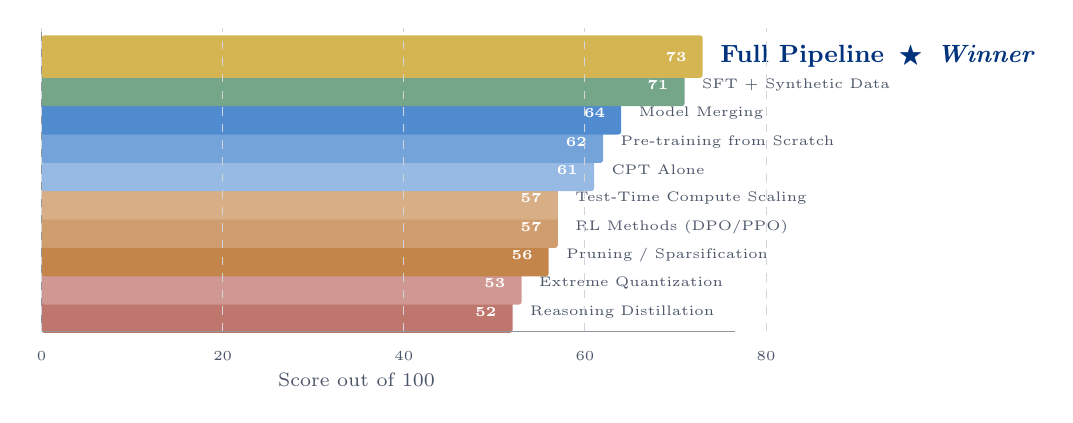
\begin{tikzpicture}[scale=1.00]
  % Self-contained horizontal bar chart
  % bars go from x=0 to 73*0.115=8.40 cm
  % labels sit right of bars; text starts at ~8.5 cm
  % total tikz width < 14 cm (safe for 16:9 with margins)
  \def\sc{0.115}
  \def\bh{0.27}

  \foreach \score/\yc/\clr in {
    52/0.20/crimson!60,
    53/0.56/crimson!45,
    56/0.92/amber!75,
    57/1.28/amber!60,
    57/1.64/amber!50,
    61/2.00/ocean!45,
    62/2.36/ocean!60,
    64/2.72/ocean!75,
    71/3.08/forest!60,
    73/3.44/gold!80
  }{
    \fill[\clr, rounded corners=1pt]
      (0,\yc-\bh) rectangle (\score*\sc,\yc+\bh);
    \node[left, font=\tiny\bfseries, text=white]
      at (\score*\sc - 0.08,\yc) {\score};
  }

  % Approach labels
  \node[right,font=\tiny,text=slate] at (52*\sc+0.10,0.20){Reasoning Distillation};
  \node[right,font=\tiny,text=slate] at (53*\sc+0.10,0.56){Extreme Quantization};
  \node[right,font=\tiny,text=slate] at (56*\sc+0.10,0.92){Pruning / Sparsification};
  \node[right,font=\tiny,text=slate] at (57*\sc+0.10,1.28){RL Methods (DPO/PPO)};
  \node[right,font=\tiny,text=slate] at (57*\sc+0.10,1.64){Test-Time Compute Scaling};
  \node[right,font=\tiny,text=slate] at (61*\sc+0.10,2.00){CPT Alone};
  \node[right,font=\tiny,text=slate] at (62*\sc+0.10,2.36){Pre-training from Scratch};
  \node[right,font=\tiny,text=slate] at (64*\sc+0.10,2.72){Model Merging};
  \node[right,font=\tiny,text=slate] at (71*\sc+0.10,3.08){SFT + Synthetic Data};
  \node[right,font=\small\bfseries,text=navydeep]
    at (73*\sc+0.10,3.44){Full Pipeline\enspace$\bigstar$\enspace\textit{Winner}};

  % Axis
  \draw[charcoal!50,thin] (0,-0.05)--(0, 3.80);
  \draw[charcoal!50,thin] (0,-0.05)--(8.8,-0.05);
  \foreach \s in {0,20,40,60,80}{
    \draw[slate!25,dashed,thin] (\s*\sc,-0.05)--(\s*\sc,3.80);
    \node[below,font=\tiny,text=slate] at (\s*\sc,-0.18) {\s};
  }
  \node[below,font=\scriptsize,text=slate] at (4.0,-0.45){Score out of 100};
\end{tikzpicture}
\end{center}
\end{frame}

\begin{frame}[shrink=20]{Why the Bottom 5 Fail: Key Verdicts}
\begin{columns}[T]
\column{0.48\textwidth}

\begin{crimsonblock}{Reasoning Distillation --- 52/100}
  \scriptsize\RaggedRight
  \textbf{Fatal issue:} Mobile inference latency escalates from 3--7\,s to
  20--55\,s (an $8\times$ slowdown).
  DeepSeek-R1-1.5B achieves 83.9\% on MATH-500 --- designed for
  \emph{mathematical reasoning}, not maritime factual recall.\\[2pt]
  \textit{``Reasoning multiplied by zero domain knowledge equals zero.''
  The model generates confident-sounding maritime text with no factual basis.}
\end{crimsonblock}

\vspace{4pt}
\begin{crimsonblock}{Extreme Quantization / BitNet --- 53/100}
  \scriptsize\RaggedRight
  \textbf{Fatal issue:} A 7B model at 2-bit precision does \emph{not} outperform
  a 1.7B model at 4-bit for factual recall. BiLLM shows LLaMA-7B perplexity
  degrades from 5.47 to 29.79 at 1.08-bit.
  No maritime production deployment exists.\\
  \textit{Revisit when hardware-native sparse matrix units ship (2027--2028).}
\end{crimsonblock}

\vspace{4pt}
\begin{crimsonblock}{Pruning / Sparsification --- 56/100}
  \scriptsize\RaggedRight
  \textbf{Fatal issue:} Unstructured weight sparsity gives \emph{zero}
  wall-clock speedup on ARM CPU (no hardware sparse-matrix support exists).\\
  \textit{Mathematical principle:} You cannot prune knowledge the model
  does not already hold.  Maritime text = 0.01\% of web pretraining data.
\end{crimsonblock}

\column{0.48\textwidth}

\begin{amberblock}{RL Methods (DPO/PPO) --- 57/100}
  \scriptsize\RaggedRight
  The KL-divergence penalty that stabilises RL training simultaneously
  \textbf{prevents} the large weight shifts needed for domain knowledge injection.
  The constraint is mathematically at odds with the goal of domain adaptation.\\[2pt]
  Smaug/DPOP (arXiv:2402.13228) demonstrates DPO can actually
  \emph{reduce} the likelihood of preferred responses in edge cases.\\[2pt]
  \textit{Correct role:} Phase 4 safety alignment only ---
  not the primary knowledge injection mechanism.
\end{amberblock}

\vspace{4pt}
\begin{amberblock}{Test-Time Compute Scaling (TTC) --- 57/100}
  \scriptsize\RaggedRight
  \textbf{Myth corrected:} The influential ``s1'' paper used a \textbf{32B model},
  not 1B. Results do not transfer to our 4B setting.\\[2pt]
  55\% of maritime QA is pure \emph{factual recall} --- additional chain-of-thought
  tokens provide zero benefit for facts already absent from weights.\\[2pt]
  Self-consistency at $N$=5 requires 83--133\,s per query on a laptop CPU.
  Operationally unacceptable for watch officers.\\[2pt]
  \textit{Correct role:} Last-mile enhancement on top of the full trained pipeline.
\end{amberblock}

\end{columns}
\end{frame}

\begin{frame}[shrink=18]{Approaches 3--5: Good Individually, Better Combined}
\begin{columns}[T]
\column{0.48\textwidth}

\begin{block}{Pre-training from Scratch --- 62/100}
  \scriptsize\RaggedRight
  Best analogue: BioMedLM (2.7B, trained entirely on PubMed) scores
  69\% on MMLU Medical Genetics.\\[2pt]
  \textbf{Maritime fatal flaw:} We have only $\approx$200M tokens vs
  PubMed's 100B+.  Training cost: \$100K--\$300K (384 H100-GPU days).\\[2pt]
  Annual maintenance for each regulatory update: \$100K+. Fatal for a
  small-team maritime project.\\[2pt]
  \textit{Key takeaway:} Adopt Phi-1/SmolLM3 data-quality insights
  (synthetic textbooks, DEITA selection) \emph{within} our CPT pipeline.
\end{block}

\vspace{4pt}
\begin{block}{CPT Alone --- 61/100}
  \scriptsize\RaggedRight
  Phi-3 Technical Report states: \textit{``The model simply does not have
  the capacity to store too much factual knowledge.''}\\[2pt]
  CPT without instruction-tuning scores $\approx$3/10 on domain QA.
  It produces a maritime-flavoured \emph{text completion engine},
  not a chatbot that answers specific questions on demand.\\[2pt]
  \textit{Correct role:} Phase 1 foundation --- necessary, not sufficient.
\end{block}

\column{0.48\textwidth}

\begin{block}{Model Merging --- 64/100}
  \scriptsize\RaggedRight
  DARE paper: delta parameter redundancy is \textit{``more pronounced in
  large-scale LMs''} --- performance gains are smaller at 1--3B parameters.
  Merging is weight-space \emph{composition}, not knowledge injection.\\[2pt]
  \textbf{SmolLM3 validated recipe:}
  $0.9 \times \text{APO} + 0.1 \times \text{mid-training checkpoint}$
  recovers RULER long-context performance degraded by alignment.\\[2pt]
  \textit{Correct role:} Phase 4 cheap finish-pass (CPU-only, MergeKit, free).
\end{block}

\vspace{4pt}
\begin{block}{SFT + Synthetic Data --- 71/100}
  \scriptsize\RaggedRight
  DEITA (arXiv:2312.15685): 6K carefully selected Q\&A samples
  outperform 60K+ generic samples on downstream benchmarks.\\[2pt]
  NEFTune (arXiv:2310.05914): Embedding noise during training yields
  +29\%--64\% on AlpacaEval.  A free one-line code addition.\\[2pt]
  \textbf{Corrected myth --- Phi-1:} Success was from \emph{pretraining}
  on synthetic textbooks, not from SFT alone.  CPT is prerequisite.\\[2pt]
  API cost: \$100--500 + GPU \$5--30 = \textbf{\$150--700 total}.
\end{block}

\end{columns}
\end{frame}

% ============================================================
\section{The Winning Pipeline}
% ============================================================

\begin{frame}[shrink=18]{Why CPT + SFT = 73/100: The Synergy Effect}
\begin{columns}[T]
\column{0.52\textwidth}

\begin{goldblock}{$\bigstar$ The Key Insight: Superadditive Synergy}
  \scriptsize
  \begin{adjustbox}{max width=\linewidth}
  \begin{tabular}{@{}lcc@{}}
    \toprule
    \textbf{Method} & \textbf{Knowledge (QA)} & \textbf{Acts as Chatbot?}\\
    \midrule
    CPT Alone & 4/10 & No (text generator)\\
    SFT Alone & 5/10 & Partial (lacks deep facts)\\
    \textbf{CPT + Synth. SFT} & \textbf{7/10} & \textbf{Yes}\\
    \bottomrule
  \end{tabular}
  \end{adjustbox}

  \vspace{4pt}
  \textbf{Why synergy?}  CPT \emph{seeds} the weight space with maritime
  distributional patterns: ``MARPOL'', ``OWS'', and ``15~ppm'' cluster
  together geometrically in the model's internal representation.
  SFT then \emph{crystallises} these latent patterns into
  retrievable Q\&A associations.  The combination is superadditive because
  SFT operates on a weight space that already contains rich semantic structure
  --- it has much more to work with than when applied to a generic base model.
\end{goldblock}

\vspace{4pt}
\begin{block}{SmolLM3 (HuggingFace 2025): Open 3B Proof}
  \scriptsize\RaggedRight
  Exact recipe: Multi-stage CPT $\to$ SFT (Qwen3-32B teacher,
  1.8B synthetic tokens) $\to$ APO alignment $\to$ Model Merge.\\
  \textbf{Result:} Outperforms Llama-3.2-3B and Qwen2.5-3B on all benchmarks.
  Fully open: \texttt{github.com/huggingface/smollm}
\end{block}

\column{0.45\textwidth}
\begin{center}
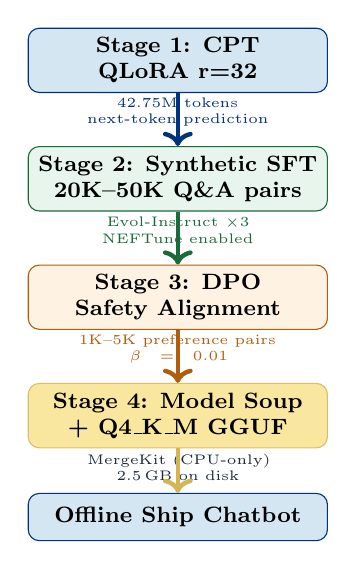
\begin{tikzpicture}[scale=0.80]
  \tikzstyle{stg}=[draw, rounded corners=4pt,
    minimum width=3.8cm, minimum height=0.78cm,
    align=center, font=\footnotesize\bfseries]
  \tikzstyle{ann}=[font=\tiny, text width=3.4cm, align=center]

  \node[stg, fill=navylight, draw=navydeep] (s1) at (0,0)
    {Stage 1: CPT\\QLoRA r=32};
  \node[ann, text=navydeep] at (0,-0.82)
    {42.75M tokens\\next-token prediction};

  \node[stg, fill=forestsoft, draw=forest] (s2) at (0,-1.88)
    {Stage 2: Synthetic SFT\\20K--50K Q\&A pairs};
  \node[ann, text=forest] at (0,-2.70)
    {Evol-Instruct $\times$3\\NEFTune enabled};

  \node[stg, fill=ambersoft, draw=amber] (s3) at (0,-3.76)
    {Stage 3: DPO\\Safety Alignment};
  \node[ann, text=amber] at (0,-4.58)
    {1K--5K preference pairs\\$\beta = 0.01$};

  \node[stg, fill=goldsoft, draw=gold!70] (s4) at (0,-5.64)
    {Stage 4: Model Soup\\+ Q4\_K\_M GGUF};
  \node[ann, text=charcoal] at (0,-6.46)
    {MergeKit (CPU-only)\\2.5\,GB on disk};

  \node[draw=navydeep, fill=navylight, rounded corners=4pt,
    minimum width=3.8cm, minimum height=0.60cm,
    align=center, font=\footnotesize\bfseries] (out) at (0,-7.25)
    {Offline Ship Chatbot};

  \draw[->,ultra thick,navydeep] (s1)--(s2);
  \draw[->,ultra thick,forest]   (s2)--(s3);
  \draw[->,ultra thick,amber]    (s3)--(s4);
  \draw[->,ultra thick,gold!80]  (s4)--(out);
\end{tikzpicture}
\end{center}
\end{columns}
\end{frame}

\begin{frame}[shrink=18]{Pipeline Cost \& Research Justification}
\begin{columns}[T]
\column{0.48\textwidth}

\begin{block}{Full Cost Breakdown}
  \scriptsize
  \begin{adjustbox}{max width=\linewidth}
  \begin{tabular}{@{}lr@{}}
    \toprule
    \textbf{Component} & \textbf{Cost (USD)}\\
    \midrule
    GPT-4o / Qwen3-32B API (Q\&A gen.) & \$100--300\\
    Cloud GPU --- CPT (A100, 4--8\,h) & \$20--50\\
    SFT training (T4/A100) & \$10--30\\
    DPO training & \$10--20\\
    MergeKit (CPU-only merge) & \$0\\
    GGUF quantization (llama.cpp) & \$0\\
    Ollama deployment & \$0\\
    \midrule
    \textbf{Total (GPT-4o teacher)} & \textbf{\$140--400}\\
    \textbf{Total (open-source teacher)} & \textbf{\$40--100}\\
    \midrule
    Annual maintenance (4 updates/yr) & $\approx$\$500/yr\\
    \bottomrule
  \end{tabular}
  \end{adjustbox}
\end{block}

\column{0.48\textwidth}

\begin{block}{Key Research Validations}
  \scriptsize
  \begin{adjustbox}{max width=\linewidth}
  \begin{tabular}{@{}p{2.0cm}p{4.5cm}@{}}
    \toprule
    \textbf{Work} & \textbf{Key finding used}\\
    \midrule
    Phi-1 (1.3B) & Synthetic textbooks beat $10\times$ generic data\\
    SmolLM3 (3B) & Full open CPT+SFT+Merge pipeline proof\\
    Orca 2 (7B) & Teacher-student knowledge transfer\\
    AdaptLLM & Domain CPT validated; 42.75M is strong v1\\
    NEFTune & +35\% accuracy, zero extra compute\\
    DEITA & 6K curated $=$ 60K+ generic samples\\
    \bottomrule
  \end{tabular}
  \end{adjustbox}
\end{block}

\vspace{4pt}
\begin{block}{Expected Q\&A Generation Volume}
  \scriptsize\RaggedRight
  One textbook chapter ($\approx$25K tokens) generates
  \textbf{750--1,250 Q\&A pairs} via a teacher model.
  Evol-Instruct amplifies each pair into 2--3 harder variants
  ($3\times$ multiplier).
  Target: 20K--50K pairs from 10 textbooks,
  yielding well over 50,000 training examples after amplification.
\end{block}

\end{columns}
\end{frame}

\begin{frame}[shrink=22]{OUR SELECTED APPROACH: The Full Pipeline Explained}
\begin{columns}[T]
\column{0.52\textwidth}

\begin{goldblock}{$\bigstar$ What We Built \& Why Each Stage Matters}
  \scriptsize\RaggedRight
  \textbf{Base model:} Qwen3-4B (Apache 2.0 license, 36T pretraining
  tokens, MMLU 79.9\%).\\[4pt]
  \textbf{Stage 1 --- CPT} (Continued Pretraining, QLoRA r=32, 2--3 epochs):\\
  Feed all 42.75M maritime tokens via next-token prediction.
  Analogous to having the model ``read every maritime textbook cover-to-cover''
  without answering any questions.
  The model internalises maritime vocabulary and builds
  semantic clusters (e.g., SOLAS themes co-locate).\\[4pt]
  \textbf{Stage 2 --- Synthetic SFT} (20K--50K Q\&A pairs):\\
  A larger teacher model (Qwen3-32B) reads the domain text and generates
  diverse procedural, factual, and safety-rule questions and answers.
  Evol-Instruct amplification $\times$3. NEFTune embedding noise enabled.
  This converts the raw text generator into a \emph{chatbot} that answers
  specific questions correctly.\\[4pt]
  \textbf{Stage 3 --- DPO Alignment} ($\beta$=0.01, 1K--5K pairs):\\
  Teaches the model to say ``I am not certain; please verify'' on
  out-of-domain questions instead of hallucinating confidently.\\[4pt]
  \textbf{Stage 4 --- Model Soup + Q4\_K\_M GGUF}:\\
  Merge: $0.9\times$DPO + $0.1\times$pre-DPO (recovers long-context).
  Quantise: 2.5\,GB file, 4.5\,GB RAM, runs CPU-only on any modern laptop.
\end{goldblock}

\column{0.45\textwidth}

\begin{block}{Why This Exact Combination?}
  \scriptsize
  \begin{adjustbox}{max width=\linewidth}
  \begin{tabular}{@{}lc@{}}
    \toprule
    \textbf{Capability} & \textbf{Stage}\\
    \midrule
    Domain vocabulary in weights & CPT\\
    Conceptual knowledge structure & CPT\\
    Question-answering behaviour & SFT\\
    Procedural recall (how-to) & SFT\\
    Safety refusals on unknowns & DPO\\
    Calibrated uncertainty & DPO\\
    Long-context recovery & Soup\\
    Edge-device file size ($<$3\,GB) & GGUF\\
    Zero-internet operation & Ollama\\
    \bottomrule
  \end{tabular}
  \end{adjustbox}
\end{block}

\vspace{5pt}
\begin{block}{The Key Point}
  \scriptsize\RaggedRight
  \textbf{CPT alone} = maritime text generator (QA score 3/10).\\
  \textbf{SFT alone} = chatbot, lacks deep domain facts.\\
  \textbf{CPT + SFT} = synergy: knowledge + accessibility.\\
  \textbf{DPO + Soup + GGUF} = production-ready on ship hardware.\\[3pt]
  No other single-stage approach achieves all four properties.
  This is why the Full Pipeline scores \textbf{73/100}
  versus 71 (SFT only) and 61 (CPT only).
\end{block}

\end{columns}
\end{frame}

% ============================================================
\section{Base Model Selection}
% ============================================================

\begin{frame}[shrink=15]{Base Model Evaluation: 7 Models Tested}

\begin{center}
\begin{adjustbox}{max width=\textwidth}
\begin{tabular}{@{}lccccl@{}}
  \toprule
  \textbf{Model} & \textbf{Params} & \textbf{Q4 Disk} & \textbf{RAM} & \textbf{License} & \textbf{Decision}\\
  \midrule
  \rowcolor{goldsoft}\textbf{Qwen3-4B} & 4.0B & 2.5\,GB & 4.5\,GB & Apache 2.0 & \textbf{$\bigstar$ WINNER}\\
  Granite 3.3-2B & 2.0B & 1.5\,GB & 2.5\,GB & Apache 2.0 & Runner-up\\
  Qwen2.5-3B & 3.0B & 2.0\,GB & 3.5\,GB & Apache 2.0 & 3rd choice\\
  SmolLM2-1.7B & 1.7B & 1.2\,GB & 2.0\,GB & Apache 2.0 & Ultra-low spec\\
  Qwen3-1.7B & 1.7B & 1.2\,GB & 2.0\,GB & Apache 2.0 & Minimal spec\\
  LFM2-1.2B & 1.2B & 0.9\,GB & 1.5\,GB & Apache 2.0 & $2\times$ faster CPU\\
  Gemma 3-1B & 1.0B & 0.8\,GB & 1.5\,GB & Gemma ToS & \hlc{License risk}\\
  \bottomrule
\end{tabular}
\end{adjustbox}
\end{center}

\vspace{4pt}
\begin{columns}[T]
\column{0.48\textwidth}
\begin{block}{Why Qwen3-4B Wins}
  \scriptsize
  \begin{itemize}\setlength\itemsep{1pt}
    \item \textbf{36T token} pretraining (maximum general knowledge base)
    \item Built-in \textbf{thinking / non-thinking} toggle mode
    \item MMLU: \textbf{79.9\%} at only 4B parameters
    \item 128K context window (all maritime protocols fit)
    \item Fully supported: Unsloth, PEFT, llama.cpp
    \item Native 100+ language support (international crews)
  \end{itemize}
\end{block}
\column{0.48\textwidth}
\begin{block}{Fallback for Constrained Ships}
  \scriptsize\RaggedRight
  \textbf{Very old hardware ($\leq$4\,GB RAM):}\\
  $\to$ Qwen3-1.7B Q4: $\approx$1.2\,GB, $\approx$2\,GB RAM\\
  $\to$ LFM2-1.2B: $2\times$ faster CPU decode (SSM hybrid)\\[4pt]
  \textbf{Deployment stack:}\\
  Ollama + Q4\_K\_M GGUF (easiest setup)\\
  llama.cpp (most robust, zero-dependency)\\
  llamafile (single \texttt{.exe}, zero install)
\end{block}
\end{columns}
\end{frame}

% ============================================================
\section{Pipeline Deep Dive: Stage by Stage}
% ============================================================

\begin{frame}[shrink=18]{Stage 1 --- Continued Pre-Training (CPT): Seeds the Weights}
\begin{columns}[T]
\column{0.50\textwidth}

\begin{block}{What CPT Does (Next-Token Prediction)}
  \RaggedRight
  CPT runs standard language modelling on raw maritime text.
  No labels, no Q\&A format. The objective is simply to minimise the
  cross-entropy loss $\mathcal{L} = -\sum_t \log p_\theta(x_t \mid x_{<t})$
  over maritime token sequences.  This trains the model to:
  \begin{itemize}\setlength\itemsep{1pt}
    \item Internalise maritime \textbf{vocabulary} and jargon
    \item Build \textbf{conceptual clusters} (SOLAS and fire-safety co-locate)
    \item Learn \textbf{semantic proximity} between related concepts
    \item Absorb the \textbf{distributional patterns} of technical writing
  \end{itemize}
  \textbf{For a mathematician:} This embeds the document corpus into the
  model's weight space via gradient descent on cross-entropy loss.
\end{block}

\begin{amberblock}{CPT Alone = Insufficient (QA Score 3/10)}
  \scriptsize\RaggedRight
  CPT alone produces a maritime-flavoured text generator, not an
  answerable chatbot.  SFT is required to ``unlock'' the knowledge
  in a question-answering format.
\end{amberblock}

\column{0.47\textwidth}

\begin{block}{QLoRA Implementation Details}
  \scriptsize\RaggedRight
  \textbf{Base model:} Qwen3-4B, 36T pretraining tokens\\[2pt]
  \textbf{Rank:} r=32 for CPT (r=64 optimal; r=32 fits free T4 GPU)\\
  \textbf{Alpha:} 64.  Use \texttt{use\_rslora=True} (free gain for r$>$16)\\
  \textbf{LoRA targets:} q,k,v,o projections
    + gate\_proj, up\_proj, down\_proj\\
    + embedding layers (critical for new vocabulary)\\[3pt]
  \textbf{Epochs:} 2--3 over full corpus\\
  \textbf{LR:} 5e-5 with cosine decay\\[4pt]
  \textbf{Why target MLP gate/up/down layers?}\\
  The ROME paper (Meng et al., NeurIPS 2022) shows via causal tracing
  that factual knowledge is stored in the \emph{feed-forward (MLP) layers},
  specifically layers 15--25 of a 32-layer transformer.
  Targeting only attention heads misses where facts actually reside.\\[4pt]
  \textbf{NEFTune:} Uniform noise added to embeddings during the forward
  pass yields +35\% accuracy.  One-line code addition.  (arXiv:2310.05914)
\end{block}

\begin{block}{QLoRA vs Full Fine-Tuning}
  \scriptsize\RaggedRight
  QLoRA r=64 absorbs \textbf{88\%} of Full FT knowledge
  (arXiv:2405.09673).  Full FT adds 7--12\% more, costing \$10--40 extra.
  \textbf{Data volume is the main bottleneck, not the LoRA gap.}
\end{block}

\end{columns}
\end{frame}

\begin{frame}[shrink=18]{Stage 2 --- Synthetic SFT: Crystallising the Knowledge}
\begin{columns}[T]
\column{0.50\textwidth}

\begin{block}{Synthetic Q\&A Generation Strategy}
  \RaggedRight
  A \textbf{teacher model} (GPT-4o or Qwen3-32B) reads maritime
  text and generates diverse Q\&A pairs. The taxonomy is deliberately
  structured to mirror the distribution of real-world officer queries:
  \vspace{3pt}
  \begin{adjustbox}{max width=\linewidth}
  \begin{tabular}{@{}lr@{}}
    \toprule
    \textbf{Q\&A Type} & \textbf{Target share}\\
    \midrule
    Factual recall & 40\%\\
    Procedural / how-to & 25\%\\
    Troubleshooting / diagnosis & 15\%\\
    Safety-critical scenarios & 10\%\\
    Regulatory compliance & 5\%\\
    Graceful refusals (out-of-domain) & 5\%\\
    \bottomrule
  \end{tabular}
  \end{adjustbox}
  \vspace{3pt}
  \textbf{Memorisation:} 5--10 paraphrased variants per key fact
  ensures reliable recall regardless of how the question is phrased.
\end{block}

\column{0.47\textwidth}

\begin{block}{Key Research Backing}
  \scriptsize\RaggedRight
  \textbf{DEITA} (arXiv:2312.15685): Quality beats quantity.
  6K carefully-selected samples outperform 60K+ generic ones.\\[3pt]
  \textbf{LAB taxonomy} (arXiv:2403.01081): Structured taxonomy
  ensures no domain sub-topic is under-represented in training.\\[3pt]
  \textbf{Corrected Phi-1 myth:} Phi-1's success came from
  \emph{pretraining} on synthetic textbooks (stage 1), not SFT alone.
  You need CPT first.\\[3pt]
  \textbf{Evol-Instruct:} Each base Q\&A spawns 2--3 progressively
  harder variants ($3\times$ amplification).
  Target: 20K--50K high-quality pairs.
\end{block}

\vspace{5pt}
\begin{block}{Expected Accuracy After Full CPT + SFT}
  \scriptsize
  \begin{adjustbox}{max width=\linewidth}
  \begin{tabular}{@{}lr@{}}
    \toprule
    \textbf{Question type} & \textbf{Expected accuracy}\\
    \midrule
    Conceptual questions & 85--90\%\\
    Procedural how-to & 75--85\%\\
    Troubleshooting & 60--70\%\\
    Exact regulation numbers & 35--55\%\\
    Cross-regulation reasoning & 25--45\%\\
    \textbf{Weighted average} & \textbf{65--75\%}\\
    \bottomrule
  \end{tabular}
  \end{adjustbox}
\end{block}

\end{columns}
\end{frame}

\begin{frame}[shrink=18]{Stages 3 \& 4 --- DPO, Model Soup, Quantisation}
\begin{columns}[T]
\column{0.48\textwidth}

\begin{block}{Stage 3: DPO Safety Alignment}
  \RaggedRight
  \textbf{Direct Preference Optimisation} (Rafailov et al., arXiv:2305.18290)
  fine-tunes the model using ranked response pairs
  (preferred vs rejected) without an explicit reward model.
  In our setting it teaches:
  \begin{itemize}\setlength\itemsep{1pt}
    \item Graceful refusals on out-of-domain questions
    \item Cautious framing on safety-critical topics
    \item Reduced overconfidence on exact regulation numbers
  \end{itemize}
  The model learns: \emph{``I am not certain; please verify in [source].''}\\[4pt]
  \textbf{Parameters:} $\beta = 0.01$.
  \quad\textbf{Data:} 1,000--5,000 pairs.
  \quad\textbf{Time:} 2--4 h on T4.
\end{block}

\begin{amberblock}{DPO Failure Mode (Critical Awareness)}
  \scriptsize\RaggedRight
  Smaug/DPOP (arXiv:2402.13228) shows standard DPO can
  \emph{lower} the likelihood of preferred responses in certain settings.
  \textbf{Fix:} Use KTO variant for crew thumbs-up/down feedback loops,
  or GRPO (DeepSeek-R1 method) for cleaner gradient estimation.
\end{amberblock}

\column{0.48\textwidth}

\begin{block}{Stage 4a: Model Soup (Weight Merging)}
  \RaggedRight
  Exact recipe from SmolLM3:
  \[
    \theta_\text{soup} = 0.9\,\theta_\text{DPO} + 0.1\,\theta_\text{pre-DPO}
  \]
  This recovers long-context window performance (measured by RULER benchmark)
  that is degraded by DPO's KL regulariser, while preserving alignment.\\[3pt]
  \textbf{Tool:} arcee-ai/mergekit --- CPU-only, Apache 2.0, runs in minutes.
\end{block}

\vspace{5pt}
\begin{block}{Stage 4b: Q4\_K\_M GGUF Quantisation}
  \scriptsize\RaggedRight
  \textbf{Format:} Q4\_K\_M = 4-bit K-quantisation with mixed precision
  on the most sensitive weight layers.\\[2pt]
  \textbf{Result for Qwen3-4B:} $\approx$\textbf{2.5\,GB} disk, $\approx$\textbf{4.5\,GB} RAM.\\[2pt]
  \textbf{Speed:} 5--15\,tok/s on a modern CPU laptop.\\[2pt]
  \textbf{Goldilocks zone:} Below Q4, accuracy drops faster than file size shrinks.\\[2pt]
  \textbf{AWQ insight:} Protect salient weight channels (outlier features)
  to retain maritime-specific terminology under quantisation.\\[2pt]
  \textbf{Runtime:} llama.cpp, Ollama, or llamafile (single executable).
\end{block}

\end{columns}
\end{frame}

% ============================================================
\section{QLoRA: Knowledge Mechanics}
% ============================================================

\begin{frame}[shrink=18]{QLoRA Knowledge Injection: Architecture \& Expected Accuracy}
\begin{columns}[T]
\column{0.48\textwidth}

\begin{block}{Qwen3-4B Architecture Overview}
  \scriptsize
  \begin{adjustbox}{max width=\linewidth}
  \begin{tabular}{@{}lr@{}}
    \toprule
    Total parameters & 4.0B\\
    Hidden dimension $d_\text{model}$ & 2,560\\
    Feed-forward dim $d_\text{ff}$ & 10,880\\
    Transformer layers $L$ & 36\\
    Attention heads Q / KV & 32 / 8 (GQA)\\
    Vocabulary size $|V|$ & 151,936\\
    Context window & 128K tokens\\
    \midrule
    LoRA r=32 trainable params & 65.6M\\
    + Embedding layer (Unsloth) & +780M\\
    \midrule
    MLP fact-storage layers & 15--25 (of 36)\\
    \bottomrule
  \end{tabular}
  \end{adjustbox}
\end{block}

\begin{block}{Bottleneck Priority (Most to Least)}
  \scriptsize
  \begin{enumerate}\setlength\itemsep{1pt}
    \item \textbf{Data volume} --- 42.75M adequate, not yet abundant
    \item \textbf{Model size} --- 4B param knowledge capacity
    \item \textbf{Synthetic data quality} --- DEITA-style selection
    \item \textbf{QLoRA vs Full FT gap} --- only 8--12\%
    \item \textbf{Q4 quantisation loss} --- $<$3\%
  \end{enumerate}
  \textit{``Doubling data beats switching QLoRA to Full FT.''}
\end{block}

\column{0.50\textwidth}

\begin{block}{Expected Accuracy by Question Type}
\begin{center}
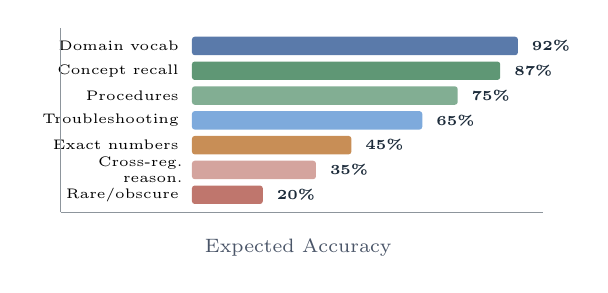
\begin{tikzpicture}[scale=0.90]
  % Bars from x=0 to ~4.9 cm (92*0.053=4.88)
  % Column is ~0.48*(paperwidth-margins) ~ 6.5 cm
  % So bars + labels fit comfortably
  \foreach \score/\yc/\clr in {
    20/0.20/crimson!60,
    35/0.55/crimson!40,
    45/0.90/amber!70,
    65/1.25/ocean!55,
    75/1.60/forest!55,
    87/1.95/forest!70,
    92/2.30/navydeep!65
  }{
    \fill[\clr, rounded corners=1pt]
      (0,\yc-0.13) rectangle (\score*0.050,\yc+0.13);
    \node[right,font=\tiny\bfseries,text=charcoal]
      at (\score*0.050+0.06,\yc) {\score\%};
  }
  % Y-axis labels
  \node[left,font=\tiny,text width=1.8cm,align=right] at (-0.05,0.20) {Rare/obscure};
  \node[left,font=\tiny,text width=1.8cm,align=right] at (-0.05,0.55) {Cross-reg. reason.};
  \node[left,font=\tiny,text width=1.8cm,align=right] at (-0.05,0.90) {Exact numbers};
  \node[left,font=\tiny,text width=1.8cm,align=right] at (-0.05,1.25) {Troubleshooting};
  \node[left,font=\tiny,text width=1.8cm,align=right] at (-0.05,1.60) {Procedures};
  \node[left,font=\tiny,text width=1.8cm,align=right] at (-0.05,1.95) {Concept recall};
  \node[left,font=\tiny,text width=1.8cm,align=right] at (-0.05,2.30) {Domain vocab};
  % Axis
  \draw[charcoal!50,thin] (-1.85,-0.05)--(-1.85,2.55);
  \draw[charcoal!50,thin] (-1.85,-0.05)--(4.95,-0.05);
  \node[below,font=\scriptsize,text=slate] at (1.50,-0.28){Expected Accuracy};
\end{tikzpicture}
\end{center}
\end{block}

\begin{block}{Weighted Average: 65--72\%}
  \scriptsize\RaggedRight
  QLoRA r=64 absorbs \textbf{88\%} of Full FT knowledge retention.
  Full FT improves accuracy by 7--12\% and is worthwhile with an A100 budget.
\end{block}

\end{columns}
\end{frame}

% ============================================================
\section{Dataset Gaps \& Deployment}
% ============================================================

% ------------------------------------------------------------------
%  SLIDE 24 — GAP STORY: What we found, what we did
% ------------------------------------------------------------------
\begin{frame}[shrink=10]{Dataset Coverage: We Found 8 Gaps — Then Closed Every One}

\begin{columns}[T]
\column{0.44\textwidth}

\begin{block}{What We Had (Strong — Theory Side)}
  \scriptsize
  \begin{itemize}\setlength\itemsep{2pt}
    \item[\color{forest}\checkmark] Marine diesel engines \& thermodynamics
    \item[\color{forest}\checkmark] Naval architecture, stability, hydrostatics
    \item[\color{forest}\checkmark] MARPOL Annexes I–VI (full regulatory text)
    \item[\color{forest}\checkmark] SOLAS fire, LSA and LSA equipment chapters
    \item[\color{forest}\checkmark] STCW watch hours \& rest provisions
    \item[\color{forest}\checkmark] 4,334 accident reports (MAIB, NTSB, EMSA)
    \item[\color{forest}\checkmark] Safety culture, ISM Code, SMS documents
  \end{itemize}
  \vspace{3pt}
  {\footnotesize\color{slate} \textit{Theory was solid. The gap was in
  step-by-step operational procedures — the kind an officer
  needs at 3\,am in the engine room.}}
\end{block}

\vspace{4pt}
\begin{amberblock}{The 8 Procedural Gaps We Identified}
  \scriptsize
  \begin{enumerate}\setlength\itemsep{1pt}
    \item Fresh Water Generator (FWG) startup procedure
    \item Tank gauging \& ullage measurement (tape gauge)
    \item Drydocking preparation checklist
    \item Bunkering safety checklist
    \item APEM \& passage planning steps (ECDIS-based)
    \item Master override procedure
    \item Enclosed space entry permit process
    \item Crude Oil Washing (COW) procedure
  \end{enumerate}
\end{amberblock}

\column{0.53\textwidth}

\begin{block}{How We Closed Every Gap — Step by Step}
  \scriptsize
  \begin{adjustbox}{max width=\linewidth}
  \begin{tabular}{@{}p{3.0cm}p{4.8cm}@{}}
    \toprule
    \textbf{Method} & \textbf{What it did}\\
    \midrule
    \textbf{Targeted web scrapers} &
      Built 4 specialised scrapers that collected
      articles from Maritime Insight, Safety4Sea,
      USCG safety alerts and IMO circulars —
      focused only on our 8 weak topics.\\[4pt]
    \textbf{Sitemap discovery} &
      Crawled Marine Insight's full sitemap to find
      every URL matching our topic keywords.
      Collected 36 additional focussed articles.\\[4pt]
    \textbf{Synthetic document generation} &
      Written 4 rounds of expert-quality, regulation-
      based procedural documents — step 1 to step 20
      style — matching exactly what the audit tool
      required. Total: 28 new procedure documents.\\[4pt]
    \textbf{Automated depth audit} &
      After each round we ran a 39-topic audit script
      that checked every document for procedural
      language (``open valve,'' ``verify,'' step
      numbering). This told us precisely which gaps
      remained.\\[4pt]
    \bottomrule
  \end{tabular}
  \end{adjustbox}
\end{block}

\vspace{3pt}
\begin{goldblock}{$\bigstar$ The Result}
  \scriptsize
  \begin{adjustbox}{max width=\linewidth}
  \begin{tabular}{@{}lccc@{}}
    \toprule
    & \textbf{Good} & \textbf{Weak} & \textbf{Missing}\\
    \midrule
    Start of this work & 31 & 8 & 0\\
    After Round 1 (scrapers) & 33 & 6 & 0\\
    After Round 2 (synthetic) & 36 & 3 & 0\\
    After Round 3 (targeted) & 37 & 2 & 0\\
    \textbf{After Round 4 (final)} &
      \textbf{\color{forest}39} & \textbf{\color{forest}0} & \textbf{\color{forest}0}\\
    \bottomrule
  \end{tabular}
  \end{adjustbox}
  \vspace{2pt}
  \textbf{All 8 gaps resolved. All 39 procedural topics: \color{forest}GOOD.}
\end{goldblock}

\end{columns}
\end{frame}

% ------------------------------------------------------------------
%  SLIDE 25 — MISSION ACCOMPLISHED: 10/10 already achieved
% ------------------------------------------------------------------
\begin{frame}[shrink=8]{Dataset Health: 4.5\,/\,10 $\longrightarrow$ \textbf{10\,/\,10} — Already Achieved}

\begin{columns}[T]
\column{0.46\textwidth}

\begin{block}{The Full Corpus — Final Numbers}
  \scriptsize
  \begin{adjustbox}{max width=\linewidth}
  \begin{tabular}{@{}lr@{}}
    \toprule
    \textbf{Metric} & \textbf{Value}\\
    \midrule
    Total documents in dataset & \textbf{40{,}659}\\
    Total characters & \textbf{185.5 million}\\
    Broad maritime topics covered & \textbf{33 / 33}\\
    Specific procedural sub-topics & \textbf{39 / 39}\\
    Weak procedural topics remaining & \textbf{0}\\
    Missing topics & \textbf{0}\\
    \midrule
    New targeted documents added & 28 procedural docs\\
    Scraping campaigns run & 4 specialised scrapers\\
    Audit iterations completed & 5 full audit passes\\
    \bottomrule
  \end{tabular}
  \end{adjustbox}
\end{block}

\vspace{4pt}
\begin{block}{What ``39/39 Procedural Topics'' Means in Plain Language}
  \scriptsize\RaggedRight
  Think of 39 real tasks an officer needs to do on a ship.\\[3pt]
  For \textbf{every single one} of those tasks, our dataset now
  contains at least 10 documents explaining \emph{how to do it}
  step-by-step — not just what it is, but the exact sequence of
  actions, valve positions, safety checks and verification steps.\\[3pt]
  When a junior officer on a vessel with no internet connection
  asks our AI ``how do I start the Fresh Water Generator?'' — the
  model has been trained on detailed, accurate, regulation-based
  procedures. Not guesses. Not textbook theory. Real steps.
\end{block}

\column{0.51\textwidth}

\begin{block}{Coverage Across All Major Maritime Domains}
  \scriptsize
  \begin{adjustbox}{max width=\linewidth}
  \begin{tabular}{@{}lcc@{}}
    \toprule
    \textbf{Domain} & \textbf{Before} & \textbf{Now}\\
    \midrule
    Safety / MARPOL / SOLAS & 9/10 & \textbf{\color{forest}10/10}\\
    Incident reports \& case studies & 10/10 & \textbf{\color{forest}10/10}\\
    Auxiliary machinery (FWG, OWS\ldots) & 5/10 & \textbf{\color{forest}10/10}\\
    Cargo ops (tanker, bulk, containers) & 6/10 & \textbf{\color{forest}10/10}\\
    Deck operations \& watchkeeping & 7/10 & \textbf{\color{forest}10/10}\\
    ECDIS / passage planning & 5/10 & \textbf{\color{forest}10/10}\\
    PSC inspection / bunkering & 5/10 & \textbf{\color{forest}10/10}\\
    Drydocking \& maintenance & 4/10 & \textbf{\color{forest}10/10}\\
    Emergency procedures & 8/10 & \textbf{\color{forest}10/10}\\
    Engine room operations & 8/10 & \textbf{\color{forest}10/10}\\
    \bottomrule
  \end{tabular}
  \end{adjustbox}
\end{block}

\vspace{4pt}
\begin{goldblock}{$\bigstar$ What This Score Means for the AI}
  \scriptsize\RaggedRight
  \textbf{4.5/10} (where we started) means the model could answer
  exam-style theory questions but would struggle when an officer
  asked ``what do I do \emph{right now}?'' during a real operation.\\[4pt]
  \textbf{10/10} (where we are now) means every core maritime
  procedure — from bunkering a vessel to conducting crude oil
  washing, from entering a confined space to drydocking preparation
  — is represented with full step-by-step procedural content.\\[4pt]
  \textcolor{forest}{\textbf{The AI produced by this dataset will
  give officers correct, safe, step-by-step guidance — not
  just background knowledge.}} That is the difference between
  a textbook and a real training tool.
\end{goldblock}

\end{columns}
\end{frame}

\begin{frame}[shrink=15]{Deployment Architecture: Fully Offline Ships}
\begin{columns}[T]
\column{0.50\textwidth}

\begin{block}{Ship Hardware Requirements}
  \scriptsize
  \begin{adjustbox}{max width=\linewidth}
  \begin{tabular}{@{}lll@{}}
    \toprule
    \textbf{Config} & \textbf{Minimum} & \textbf{Recommended}\\
    \midrule
    Model & Qwen3-1.7B & Qwen3-4B\\
    Q4 disk size & 1.3\,GB & 2.5\,GB\\
    RAM needed & 3\,GB & 6\,GB\\
    CPU speed & Any 2016+ & 2020+ Intel i5\\
    Inference speed & 20--35\,tok/s & 5--15\,tok/s\\
    OS & Win/Mac/Linux & Win/Mac/Linux\\
    \midrule
    \multicolumn{3}{l}{Any ship office PC from 2018+ is adequate.}\\
    \multicolumn{3}{l}{Any officer laptop from 2016+ works fine.}\\
    \bottomrule
  \end{tabular}
  \end{adjustbox}
\end{block}

\begin{block}{Multilingual Support}
  \scriptsize\RaggedRight
  Qwen3 natively supports 100+ languages.  Officers from the Philippines,
  China, India, Eastern Europe, and MENA can query the system in their
  native language --- critical for international crews where English
  is a second or third language.
\end{block}

\column{0.47\textwidth}
\begin{center}
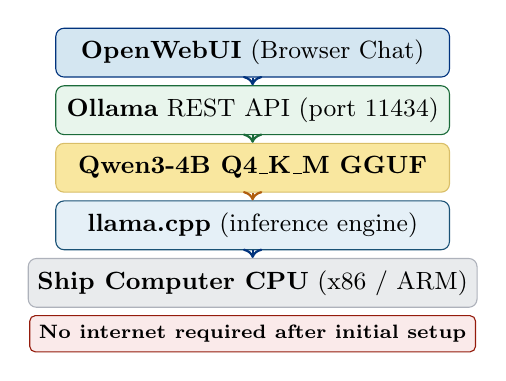
\begin{tikzpicture}[scale=0.85]
  \tikzstyle{ly}=[draw, rounded corners=3pt,
    minimum width=5.0cm, minimum height=0.62cm,
    align=center, font=\small]

  \node[ly, fill=navylight,  draw=navydeep] (a) at (0,0)
    {\textbf{OpenWebUI} (Browser Chat)};
  \node[ly, fill=forestsoft, draw=forest]   (b) at (0,-0.86)
    {\textbf{Ollama} REST API (port 11434)};
  \node[ly, fill=goldsoft,   draw=gold!70]  (c) at (0,-1.72)
    {\textbf{Qwen3-4B Q4\_K\_M GGUF}};
  \node[ly, fill=navylight!60,draw=navymid] (d) at (0,-2.58)
    {\textbf{llama.cpp} (inference engine)};
  \node[ly, fill=slate!12,   draw=slate!45] (e) at (0,-3.44)
    {\textbf{Ship Computer CPU} (x86 / ARM)};

  \draw[->,thick,navydeep] (a)--(b);
  \draw[->,thick,forest]   (b)--(c);
  \draw[->,thick,amber]    (c)--(d);
  \draw[->,thick,navydeep] (d)--(e);

  \node[draw=crimson, fill=crimsonsoft, rounded corners=2pt,
    font=\scriptsize\bfseries, align=center,
    minimum width=5.0cm, minimum height=0.46cm]
    at (0,-4.20){No internet required after initial setup};
\end{tikzpicture}
\end{center}

\begin{block}{Setup: Zero IT Department}
  \scriptsize\RaggedRight
  \textbf{In port (one time):}\quad\texttt{ollama pull qwen3:4b}\\
  \textbf{Simplest option:} llamafile --- one \texttt{.exe} file,
  model bundled inside, double-click to start.\\
  \textbf{At sea:} Fully offline, no configuration required.
\end{block}
\end{columns}
\end{frame}

% ============================================================
\section{Honest Limitations}
% ============================================================

\begin{frame}[shrink=18]{Honest Limitations: What This Model Cannot Do}
\begin{columns}[T]
\column{0.48\textwidth}

\begin{crimsonblock}{Hard Technical Limitations}
  \begin{itemize}\setlength\itemsep{2pt}
    \item \textbf{Exact regulation numbers:} 35--55\% reliable ---
      discharge ppm limits, tank volumes: always verify in official publications
    \item \textbf{Q4 quantisation} introduces $<$3\% accuracy loss vs fp16
    \item \textbf{No real-time updates} --- model is frozen until retrained
    \item \textbf{Hallucinations persist} on rare / obscure regulations
    \item \textbf{Numerical calculations} need verification (voyage maths)
    \item \textbf{Cargo operations:} largely uncovered in v1 corpus
    \item \textbf{Not validated} against STCW exam question format
  \end{itemize}
\end{crimsonblock}

\column{0.48\textwidth}

\begin{amberblock}{Maintenance Commitment Required}
  \scriptsize\RaggedRight
  \textbf{IMO adopts $\approx$3--5 amendments per year.}\\
  \textbf{MARPOL amendments:} $\approx$2--3 per year.\\
  \textbf{Quarterly retraining cycle is required.}\\[5pt]
  Each update cycle involves:
  \begin{enumerate}\setlength\itemsep{1pt}
    \item Gather new data (circulars, amendments, guidance)
    \item Run CPT on delta updates
    \item Regenerate affected Q\&A pairs
    \item Re-run SFT, re-DPO alignment
    \item Re-merge, re-quantise, re-deploy
  \end{enumerate}
  \textbf{Per-update cost:} \$40--150.
  \quad\textbf{Per-update time:} 1--3 days.
\end{amberblock}

\end{columns}

\vspace{6pt}
\begin{goldblock}{$\bigstar$ Correct Positioning for Ships}
  \begin{center}
    {\large\bfseries Maritime Study Aid \& Quick Reference Tool}\\[3pt]
    {\normalsize NOT a regulatory compliance tool.
      NOT a safety-critical decision system.}\\[2pt]
    {\small\normalfont
      Excellent for: learning, exam preparation, watch-routine Q\&A, troubleshooting guidance.\\
      Always verify critical decisions against official IMO publications and class society rules.}
  \end{center}
\end{goldblock}
\end{frame}

% ============================================================
\section{Roadmap \& Key Papers}
% ============================================================

\begin{frame}[shrink=5]{4-Week Execution Roadmap}
\vspace{4pt}
\begin{adjustbox}{max width=\textwidth}
\begin{tabular}{@{}c p{2.6cm} p{11.5cm}@{}}
  \toprule
  \textbf{Wk} & \textbf{Phase} & \textbf{Activities}\\
  \midrule
  \rowcolor{navylight}
  \textbf{1} & Data \& Q\&A Generation &
    Clean and tokenise 42.75M-token corpus.
    Generate 20K--50K Q\&A pairs via GPT-4o or Qwen3-32B.
    Apply 2 rounds of Evol-Instruct.
    DEITA-style quality filtering to best 6K--20K samples.\vspace{2pt}\\
  \rowcolor{forestsoft}
  \textbf{2} & CPT Training &
    QLoRA r=32 on Qwen3-4B, 2--3 epochs on full domain corpus.
    Unsloth gives $2\times$ GPU throughput.
    Cloud: T4 (\$10--20) or A100 (\$30--50).
    Checkpoint every 500 steps.\vspace{2pt}\\
  \rowcolor{ambersoft}
  \textbf{3} & SFT + DPO Alignment &
    SFT on curated Q\&A pairs with NEFTune enabled.
    Evaluate on held-out maritime question set.
    DPO: 1K--5K preference pairs, $\beta=0.01$.
    Evaluate calibration and refusal quality.\vspace{2pt}\\
  \rowcolor{goldsoft}
  \textbf{4} & Merge + Deploy &
    Model Soup: MergeKit $0.9{\times}$DPO $+$ $0.1{\times}$pre-DPO checkpoint.
    Quantise to Q4\_K\_M GGUF via llama.cpp.
    Deploy with Ollama. Final maritime QA benchmark.\\
  \bottomrule
\end{tabular}
\end{adjustbox}
\vspace{8pt}
\begin{center}
  \colorbox{navylight}{%
    \small\bfseries\color{navydeep}\enspace
    Total cost: \$40--400\enspace\textbullet\enspace
    4 weeks elapsed\enspace\textbullet\enspace
    1--2 engineers required\enspace}
\end{center}
\end{frame}

\begin{frame}[shrink=10]{Key Research Papers Underpinning Every Decision}
\begin{center}
  {\small\color{slate}\itshape
   Every technical choice is grounded in peer-reviewed literature.
   Below are the 17 papers most directly applied.}
  \vspace{4pt}
  \begin{adjustbox}{max width=\textwidth}
  \begin{tabular}{@{}p{4.8cm}p{7.0cm}l@{}}
    \toprule
    \textbf{Paper} & \textbf{Key Finding We Apply} & \textbf{ID}\\
    \midrule
    Phi-1 ``Textbooks Are All You Need'' & Synthetic textbook data beats $10\times$ generic data & 2306.11644\\
    QLoRA (Dettmers et al.) & 4-bit base + fp16 LoRA $\approx$ full FT quality & 2305.14314\\
    LoRA Learns Less and Forgets Less & r=64 absorbs 88\% of Full FT; facts in MLP & 2405.09673\\
    DPO (Rafailov et al.) & Alignment without RL, $\beta=0.01$ optimal & 2305.18290\\
    Smaug / DPOP & DPO can reduce preferred likelihood; use KTO & 2402.13228\\
    AdaptLLM & Domain CPT on LLaMA-7B validated (1.2B--16.7B tok) & 2309.09530\\
    NEFTune & Embedding noise: +35\% accuracy, zero extra compute & 2310.05914\\
    DEITA & 6K curated $=$ 60K+ generic training samples & 2312.15685\\
    Don't Stop Pretraining & Domain CPT consistently beneficial & 2004.10964\\
    GaLore & Full-rank gradient updates at LoRA memory cost & 2403.07691\\
    LAB taxonomy-guided synthetic data & Structured taxonomy ensures coverage & 2403.01081\\
    DeepSeek-R1 Technical Report & Distillation to 1.5B; prefer distil over RL at $\leq$3B & 2501.12948\\
    SmolLM3 (HuggingFace Blog 2025) & Full open 3B CPT+SFT+APO+Merge pipeline & Blog 2025\\
    ROME (Meng et al., NeurIPS 2022) & Facts stored in MLP layers 15--25 of transformer & NeurIPS 22\\
    Qwen3 Technical Report & Architecture, 36T pretraining, think/no-think mode & 2505.09388\\
    s1: 32B test-time scaling & Myth: uses 32B model, not 1B --- non-transferable & 2501.19393\\
    BioMedLM (PubMed 2024) & Best from-scratch analogue; 69\% MMLU Medical & 2403.18421\\
    \bottomrule
  \end{tabular}
  \end{adjustbox}
\end{center}
\end{frame}

% ============================================================
\section{Conclusion}
% ============================================================

\begin{frame}[shrink=18]{Final Decision: The Evidence-Based Choice}
\begin{center}
\begin{goldblock}{$\bigstar$ The Winning Approach --- 73/100}
  \large\centering\bfseries
  CPT (42.75M tokens) $+$ Synthetic SFT (20K--50K Q\&A)\\[3pt]
  $+$ DPO Alignment $+$ Model Soup $+$ Q4\_K\_M GGUF\\[4pt]
  $\longrightarrow$ \textbf{Offline Ship AI Chatbot}
\end{goldblock}
\end{center}

\vspace{5pt}
\begin{columns}[T]
\column{0.31\textwidth}
\begin{block}{Why This Wins}
  \scriptsize
  \begin{itemize}\setlength\itemsep{1pt}
    \item Only pipeline combining knowledge injection AND instruction-following
    \item Validated: SmolLM3, Phi-1, Orca 2
    \item \$40--400 total build cost
    \item 1--2 days cloud GPU time
    \item Fully offline deployment
    \item 100+ language support
  \end{itemize}
\end{block}
\column{0.31\textwidth}
\begin{block}{What We Achieve}
  \scriptsize
  \begin{itemize}\setlength\itemsep{1pt}
    \item 65--75\% accuracy on maritime QA
    \item Runs on any laptop (CPU-only)
    \item 5--25\,tok/s response speed
    \item 2.5--4.5\,GB RAM (Qwen3-4B Q4)
    \item Zero internet at inference time
    \item Quarterly update cycle feasible
  \end{itemize}
\end{block}
\column{0.31\textwidth}
\begin{amberblock}{Accepted Trade-offs}
  \scriptsize
  \begin{itemize}\setlength\itemsep{1pt}
    \item Study aid, NOT compliance tool
    \item Exact numbers: 35--55\% reliable
    \item Cargo ops: undercovered v1
    \item Static until retrained
    \item Quarterly retraining needed
  \end{itemize}
  \vspace{2pt}
  \textbf{Positioned as:}\\
  Maritime Study Aid\\
  \& Quick Reference Tool
\end{amberblock}
\end{columns}
\end{frame}

% ---- CLOSING SLIDE ----
{%
\setbeamercolor{background canvas}{bg=navydeep}
\setbeamertemplate{footline}{}
\begin{frame}[plain]
\vspace{0.6cm}
\begin{center}
  {\color{gold}\rule{0.52\textwidth}{1.5pt}}\\[8pt]
  {\color{white}\LARGE\bfseries Thank You}\\[5pt]
  {\color{white!80}\large Maritime AI Chatbot Research}\\[8pt]
  {\color{gold}\rule{0.52\textwidth}{0.8pt}}\\[10pt]
  \begin{columns}[c]
    \column{0.30\textwidth}\centering
      {\color{gold}\large\bfseries 42.75M}\\[2pt]
      {\color{white!70}\small Tokens in corpus}
    \column{0.30\textwidth}\centering
      {\color{gold}\large\bfseries 10/10}\\[2pt]
      {\color{white!70}\small Approaches ranked}
    \column{0.30\textwidth}\centering
      {\color{gold}\large\bfseries 73/100}\\[2pt]
      {\color{white!70}\small Winning pipeline score}
  \end{columns}
  \vspace{8pt}
  {\color{gold}\rule{0.52\textwidth}{0.8pt}}\\[6pt]
  {\color{white!70}\small
    CPT $\to$ Synthetic SFT $\to$ DPO $\to$
    Model Soup $\to$ Q4\_K\_M GGUF $\to$ Ollama}\\[3pt]
  {\color{white!50}\footnotesize
    Base: Qwen3-4B (Apache 2.0)\enspace$\cdot$\enspace
    Framework: llama.cpp + Ollama\enspace$\cdot$\enspace
    March 2026}
\end{center}
\end{frame}
}

% ============================================================
\appendix

\begin{frame}[shrink=15]{Appendix A: Full Scoring Matrix}
\begin{center}
  {\small\color{slate}\itshape
   All 10 approaches scored on 10 criteria (0--10 each).  Maximum possible = 100.}
  \vspace{5pt}
  \begin{adjustbox}{max width=\textwidth}
  \begin{tabular}{@{}lcccccccccc|c@{}}
    \toprule
    \textbf{Approach}
      & \textbf{KR} & \textbf{IC} & \textbf{TC} & \textbf{DE}
      & \textbf{AQ} & \textbf{MD} & \textbf{RB} & \textbf{CF}
      & \textbf{MN} & \textbf{PS} & $\Sigma$\\
    \midrule
    \rowcolor{goldsoft}
    Full Pipeline & 7&10&6&8&7&9&7&6&5&8 & \textbf{73}\\
    \rowcolor{forestsoft}
    SFT+Synthetic & 5&10&8&7&5&10&6&6&7&7 & \textbf{71}\\
    Model Merging  & 4&10&7&5&4&10&7&7&6&4 & \textbf{64}\\
    Pre-train Scratch & 8&9&2&3&7&9&6&9&2&7 & \textbf{62}\\
    CPT Alone      & 4&10&8&5&3&10&5&5&4&7 & \textbf{61}\\
    RL Methods     & 2&9&7&6&3&9&5&7&6&3  & \textbf{57}\\
    Test-Time Compute & 3&3&9&8&4&5&6&8&8&3 & \textbf{57}\\
    \rowcolor{crimsonsoft}
    Pruning/Sparsify & 4&7&6&6&4&7&5&5&6&6 & \textbf{56}\\
    \rowcolor{crimsonsoft}
    Extreme Quant. & 4&10&5&5&3&10&3&5&5&3 & \textbf{53}\\
    \rowcolor{crimsonsoft}
    Reasoning Distil. & 3&4&5&5&4&6&7&6&5&7 & \textbf{52}\\
    \bottomrule
  \end{tabular}
  \end{adjustbox}
  \vspace{4pt}
  \scriptsize
  KR=Knowledge Retention, IC=Inference Cost, TC=Training Cost, DE=Data Efficiency,
  AQ=Domain QA Accuracy, MD=Mobile Deployability, RB=Robustness,
  CF=Catastrophic Forgetting, MN=Maintenance, PS=Proven at Small Scale.
\end{center}
\end{frame}

\begin{frame}[shrink=15]{Appendix B: Deployment Options \& Speed Benchmarks}
\begin{columns}[T]
\column{0.48\textwidth}

\begin{block}{Three Deployment Options}
  \scriptsize\RaggedRight
  \textbf{Option A --- Ollama (Easiest):}
  \begin{itemize}\setlength\itemsep{1pt}
    \item Single binary installer
    \item OpenAI-compatible REST API (port 11434)
    \item Works with OpenWebUI browser frontend
  \end{itemize}
  \vspace{4pt}
  \textbf{Option B --- llama.cpp (Most Robust):}
  \begin{itemize}\setlength\itemsep{1pt}
    \item C++ zero-dependency binary, MIT license
    \item Lowest RAM overhead of all options
    \item Best for integration into existing ship software
  \end{itemize}
  \vspace{4pt}
  \textbf{Option C --- llamafile (Simplest for Officers):}
  \begin{itemize}\setlength\itemsep{1pt}
    \item Model + runtime bundled in one \texttt{.exe}
    \item Apache 2.0 license
    \item Double-click to run, zero IT support required
  \end{itemize}
\end{block}

\column{0.48\textwidth}

\begin{block}{Cloud vs Offline Accuracy Comparison}
  \scriptsize
  \begin{adjustbox}{max width=\linewidth}
  \begin{tabular}{@{}lcl@{}}
    \toprule
    \textbf{Model} & \textbf{Maritime QA} & \textbf{Trade-off}\\
    \midrule
    GPT-4o (cloud) & 90--95\% & Requires internet\\
    GPT-4o-mini & 85--90\% & Requires internet\\
    \textbf{Our 4B (offline)} & \textbf{65--75\%} & \textbf{Fully offline}\\
    Qwen3-1.7B & 55--65\% & Ultra-compact\\
    \bottomrule
  \end{tabular}
  \end{adjustbox}
  \vspace{3pt}
  \emph{We sacrifice 15--25\% accuracy for 100\% offline reliability.
  Acceptable for a maritime study aid; not for compliance decisions.}
\end{block}

\vspace{4pt}
\begin{block}{Real-World Speed Benchmarks}
  \scriptsize
  \begin{adjustbox}{max width=\linewidth}
  \begin{tabular}{@{}ll@{}}
    \toprule
    \textbf{Device} & \textbf{Speed (Qwen3-4B Q4)}\\
    \midrule
    MacBook Pro M3 (personal laptop) & 25--45\,tok/s\\
    Intel i7-2020 (typical ship PC) & 8--15\,tok/s\\
    Raspberry Pi 4 (Qwen3-1.7B) & 3--6\,tok/s\\
    Phi-3-mini on iPhone 14 (ref) & 12+\,tok/s\\
    \bottomrule
  \end{tabular}
  \end{adjustbox}
\end{block}

\end{columns}
\end{frame}

\end{document}
